%%%%%%%%%%%%%%%%%%%%%%%%%%%%%%%%%%%%%%%%%
% University/School Laboratory Report
% LaTeX Template
% Version 3.0 (4/2/13)
%
% This template has been downloaded from:
% http://www.LaTeXTemplates.com
%
% Original author:
% Linux and Unix Users Group at Virginia Tech Wiki 
% (https://vtluug.org/wiki/Example_LaTeX_chem_lab_report)
%
% License:
% CC BY-NC-SA 3.0 (http://creativecommons.org/licenses/by-nc-sa/3.0/)
%
%%%%%%%%%%%%%%%%%%%%%%%%%%%%%%%%%%%%%%%%%

%----------------------------------------------------------------------------------------
%	PACKAGES AND DOCUMENT CONFIGURATIONS
%----------------------------------------------------------------------------------------

\documentclass{article}

% \usepackage[version=3]{mhchem} % Package for chemical equation typesetting
%\usepackage{siunitx} % Provides the \SI{}{} command for typesetting SI units

\usepackage{graphicx} % Required for the inclusion of images
\usepackage{epstopdf} % Include .eps files
\usepackage[hidelinks]{hyperref} % For inclusion of urls
\usepackage{mathtools}	% For inclusion of \align environment (instead of eqnarray)
\usepackage{listings} % for Source Code Listing
\usepackage{color}	  % Colors
\usepackage{caption}  % Captions
\usepackage{subcaption}  % Subfigure Captions

\usepackage{rotating, booktabs} % For table formatting

\usepackage{enumitem} % Customize enumerate environment
\usepackage{appendix} % For making an Appendix
\usepackage{natbib} 	% Bibliography styles
%\setlength\parindent{0pt} % Removes all indentation from paragraphs

% \renewcommand{\labelenumi}{\alph{enumi}.} % Make numbering in the enumerate environment by letter rather than number (e.g. section 6)

%\usepackage{times} % Uncomment to use the Times New Roman font

\definecolor{mygreen}{rgb}{0,0.6,0}
\definecolor{mygray}{rgb}{0.5,0.5,0.5}

\lstset{
	basicstyle = \footnotesize,
	commentstyle = \color{mygreen},
	frame = single,
	numbers = left,
	tabsize = 2,
	breaklines = true
}


%----------------------------------------------------------------------------------------
%	DOCUMENT INFORMATION
%----------------------------------------------------------------------------------------

\title{Diffusion Limited Aggregation: Crystal Formation} % Title

\author{Vinay Rajur (vsr7)} % Author name

%\date{\today} % Date for the report
\date{December 19, 2013} % Date for the report

\begin{document}

\maketitle % Insert the title, author and date

\begin{center}
\begin{tabular}{l r}
Course: & AEP 4380 \\ % Date the experiment was performed
Instructor: & Professor Kirkland % Instructor/supervisor
\end{tabular}
\end{center}

% If you wish to include an abstract, uncomment the lines below
\begin{abstract}
This paper explores the properties of crystal formation using a Diffusion Limited Aggregation (DLA) Model. Through simulating various conditions under which crystals and other aggregates may form, several classifications were defined based on relative clustering, apparent symmetries and characteristic visual cues. Limitations of the DLA Model and the classification of crystals are also discussed.\\
\end{abstract}

%----------------------------------------------------------------------------------------
%	SECTION 1
%----------------------------------------------------------------------------------------

\section{Introduction}

The presence of pattern formation in nature, the seemingly impossible feat of creating order from random and disordered processes, is an inherently captivating and intriguing phenomenon. For scientists, it is a topic of great interest as well, and creating models to describe these processes has the potential to reveal the much of nature's inner workings.

One model in particular that has received a great deal attention over the past couple decades is the Diffusion-Limited Aggregation (DLA) Model, a deceptively simple stochastic growth model that accurately simulates the growth patterns of objects ranging from snowflakes to entire galaxies. Originally proposed by Witten and Sander in 1981, they developed a simple algorithm to model the growth of clusters in aerosols using diffusion and Brownian motion as the main transport process governing particle behavior \cite{originalDLA}. 

The simplest form of their model starts with an immobile seed particle located at the center of a lattice. At each iteration, a random walker particle is released into the lattice until it reaches a grid spot adjacent to an immobile particle, at which point, the walker becomes immobilized as well. This process is repeated for a set number of particles and the end result is a fractal (self-similar) growth pattern, which is seen in many natural aggregates as well (one such example is shown in Fig. \ref{DLA_Cluster}). The complex patterns this model is capable of producing, the accuracy of its results and the simplicity in implementing this algorithm are the key advantages for the DLA Model, and this has been the major influence and drawn significant attention in further researching the additional applications of this type of simulation.

\begin{figure}[h]
\begin{center}
	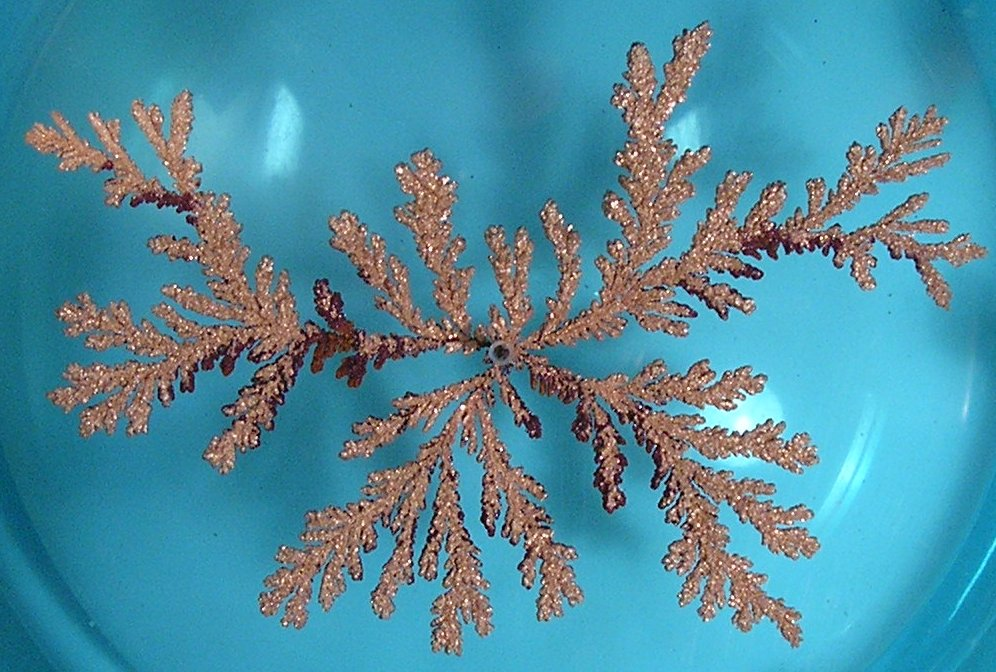
\includegraphics[width=0.65\textwidth]{DLA_Cluster}
	\caption{A DLA Cluster of Copper Sulfate grown by electrodeposition. (Image Courtesy: 
	\url{http://upload.wikimedia.org/wikipedia/commons/b/b8/DLA_Cluster.JPG)}}
	\label{DLA_Cluster}
\end{center}
\end{figure}

Over the years, many variations of this simple DLA algorithm have been developed to model a vast array of physical growth processes. For example, varying the lattice geometry has allowed researchers to accurately simulate snowflake growth \cite{nitt}, or even through creating a distribution of seed particles and varying the diffusion properties, one can model the growth of blood vessels in the human retina \cite{retina}; clearly there is a wide variety of parameters to expand upon and manipulate with this algorithm. Therefore to simplify, this paper focuses on the development of an accurate 2D model for crystal growth using a continuous surface (i.e. no lattice). Furthermore by incorporating and testing several different sticking probability distributions, I aim to develop generalized classes for different types of aggregate structures based upon fractal dimension, number volume density, apparent symmetries and characteristic visual cues. Additionally, I seek to determine the feasibility of and minimum criteria needed for defining these classes of aggregates.

 
%----------------------------------------------------------------------------------------
%	SECTION 2
%----------------------------------------------------------------------------------------

\section{Theory}


\subsection{Random Walk Behavior in the DLA Model:}

As the name suggests, the motion of particles in the DLA Model is assumed to be governed entirely by diffusion through the containing medium. The density distribution $U(\rho,t)$ in cylindrical coordinates is given by the equation:

\begin{equation}
	\frac{\partial U(\rho,t)}{\partial t} = D \nabla^2 U(\rho,t) 
	\label{fick}
\end{equation}

where D is the diffusion constant, which gives insight into the characteristic length and velocity of particle motion. Solving Eq. \ref{fick} for $U(\rho,t)$ yields the result:

\begin{equation}
	U(\rho,t) = U_0 \frac{2 \pi \rho}{4 \pi Dt}e^{ \frac{\rho^2}{4Dt}}
	\label{gauss}
\end{equation}

\noindent Thus, the result for the density distribution is a Gaussian curve centered at the origin that spreads out in time (as particles diffuse farther away). Additionally, as Einstein established in a paper written in 1905, the mechanism underlying this diffusion process is the Brownian motion of particles, the seemingly random path taken by particles suspended in some solution \cite{einstein}. Therefore in the DLA Model, the movement of the unbound aggregate particles can be simulated by a random walk, adhering the ``Diffusion-Limited'' constraint of the model. 

One caveat to consider, however, is that when fixing the seed particle at the center of the coordinate system, we are essentially shifting into the seed particle's frame of motion, and since a general model for DLA should assume that the seed is also undergoing Brownian motion, one would assume that the motion of all other particles must be transformed into the seed's frame of reference as well. Fortunately, since the motion of one Brownian particle is independent of the motion of another, the random walk behavior of the unbound particles is preserved, and so it is still accurate to describe the motion of the unbound particles by a random walk.\\

\subsection{Sticking Probability:}

One physical variation that can be applied to the DLA Model is the inclusion of a sticking probability, or the probability that a walker will bind itself to the aggregate after coming into contact with it. A nearly infinite variety of functions can be applied to the walker particles, however, the ones used for this experiment were the following: \\

\begin{enumerate} 
	\item{Constant probability:

\begin{equation}
	p = C
\label{p:coeff}
\end{equation}

	where $C \in [0,1]$.
	\label{itm1}} \pagebreak
	\item {Probability dependent on the number of neighboring particles\\
	
\begin{equation}
	p = A - B\frac{n_1}{n_2}
\label{p:neighbor}
\end{equation}

	where $A$ and $B$ are set parameters,\\ $n_1$ is the number of particles in a $\frac{L}{2} \times \frac{L}{2}$ box around the Brownian particle,\\ $n_2$ is the number of particles in a $L \times L$ box around the Brownian particle.
	\label{itm2}}
	\item{Probability dependent on the local curvature at the point of contact \cite{vic} 
	
\begin{equation}
	p = A(n_L - n_0) + B
\label{p:curvature}
\end{equation}
	
	where $A$ and $B$ are set parameters,\\
	$n_L$ is the normalized number of particles in a $L \times L$ box (e.g. $\frac{N_L}{L^2}$)\\
	$n_0 = \frac{L-1}{2L}$ corresponds to a flat contact surface.
	\label{itm3}} 
	\end{enumerate}

\noindent Of these probability functions, the constant probability function shown in \ref{itm1} is the simplest, and physical interpretation for this is that every particle has some set likelihood of binding to the aggregate at each point of contact (and conversely there is some fixed probability of the particle continuing to diffuse as well). 

This type of probability dependence easily demonstrates the implications of including a sticking probability into our DLA Model. For a low sticking probability, random walkers will tend to pass through regions of low particle density and will more likely accumulate in regions of high particle density; therefore in this scenario aggregates will form dense clumps will appear more condensed and ``filled in''. The opposite is true for a high sticking probability, as the diffusing particles will immediately bind to any part of the aggregate that it comes into contact with. Thus, the end result in this case is a wispier, more spread out aggregate structure (see Figure \ref{sticky}). 

\begin{figure}[ht!]
\begin{center}
	\includegraphics[width=\textwidth]{sticky.eps}
	\caption{Aggregates grown with various constant sticking probability values (from left to right): $p = \left\{ 0.01, 0.1, 0.5, 1.0 \right\}$. As the probability increases, the collections tend to become more tenuous and branched, occupying larger regions of space, and the opposite is true as the sticking probability decreases. Each aggregate contains $N=1000$ particles.}
	\label{sticky}
\end{center}
\end{figure}

This concept can be extrapolated to explain the local behavior of any arbitrary sticking probability function, due to the self-similar nature of aggregates formed by DLA. Regions of low sticking probability will result in denser patterns, while regions with high sticking probability will result in more tenuous growth patterns. This local rule will always apply when considering the results produced by using other probability functions (such as the proposed functions \ref{itm2} and \ref{itm3}), and the overall impact these functions will have on the total aggregate structure stems from manipulating the locations of these regions of high and low particle density (due to manipulating the sticking probability). Thus, the properties of aggregates formed with a constant sticking probability are similar to the local probabilities of aggregates with more complex sticking probability functions. 


%----------------------------------------------------------------------------------------
%	SECTION 3
%----------------------------------------------------------------------------------------

\section{My Algorithm for Simulating 2D Crystal Growth}


\subsection{Assumptions: \label{assumptions}}

In order to simplify the implementation of the DLA Model described in this section, the following assumptions were made:

\begin{enumerate}
	\item{Simulated particles undergo simple 2D Brownian motion, thus there is no motion or aggregation in the $\hat{z}$ direction\footnote{This is not entirely true in this implementation model, since particles were allowed to overlap. This effect was small, however, except for in areas of very high particle density so the general behavior of the DLA Model was still 2 dimensional}. Additionally, particle displacements are of constant step size but with a continuous range in direction (and so particles have an approximately continuous motion).
	\label{assume1}}
	
	\item{Aggregate member particles have some attractive potential well surrounding them, inside of which walker particles are likely to bind to the aggregate. The probability of binding and the functional dependence of this potential well is described by the sticking probability.
	\label{assume2}}
	
	\item{In conjunction with \ref{assume1}, particles have no inherent directional preference in binding (circular symmetry of system).
	\label{assume3}}
	
	\item{Particles are stably bound, thus decrystallization effects (such as thermal activity, momentum transfer during binding, coulomb force interaction, etc.) are negligible.
	\label{assume4}}
	
\end{enumerate}

\noindent These assumptions, while not all are entirely physical, are still representative of a true DLA system that one would observe in an experimental setting, simplifying the implementation while preserving the behavior of the model.


\subsection{The Algorithm:}

In my implementation of DLA Model (presented in Appendix \ref{source}), I created the simulation on an arbitrary scale with the basic unit length being the particle diameter. Since Particle diameter, step size, binding radius and other parameters are all relatively defined without reference to any physical constants or absolute reference, the following implementation is a general model for Diffusion Limited Aggregation that can be applied to DLA processes on any length scale\footnote{Although the type of model I based this implementation off of was an electrodeposition model}.

For the simulations I ran, I initialized the aggregate with a single seed particle placed at the center of the coordinate system. With each iteration, a random walker particle is initialized at some point along the circumference of a circle that spans the entire aggregate, and the particle undergoes Brownian motion until it binds to the aggregate. For typical simulation with about 1000 particles and constant sticking probability $\rho \in [.25, .75]$, each particle reaches its final state after around 50,000-150,000 steps\footnote{This range of values defines the average number of steps each individual walker particle takes until it binds. Physically, these particles will move in parallel, however, this simulation is for dilute particle concentrations such that the particles can be simulated as arriving one at a time.}, although due to the nature of the algorithm, these values are subject to significant statistical fluctuations. The entire binding process a single particle undergoes is composed of two main steps:

\begin{enumerate}
	
	\item{ \textit{Diffusion}:\\
		Diffusion is the result of Brownian motion, which this model simulates by using Monte Carlo methods to generate a random walk. 		Each step the particle takes is of a fixed size, however the particle has full directional freedom; thus in this simulation, the particle has a continuous range of motion. After each step, the particle is evaluated as being either bound or not. If the particle is evaluated as unbound, it will continue to diffuse.
	\label{step1}}
	
	\item{	\textit{Binding}:\\
		Binding occurs when two conditions are met: a) the particle is within the binding radius of some member of the aggregate and b) the particle is evaluated with some probability as being bound or not (where the probability is generated from the sticking probability function). Only once both conditions are met will the particle stop diffusing and bind to the aggregate. The binding process used in this model is rather simple (perhaps overly simple) where the newly bound particle simply stops in its place. This is slightly unphysical since it allows for overlapping particles, but it can be easily remedied in future updates or implementations by simply adding in a setting method (that ``sets'' the particle in the closest position that maximizes its sticking probability). The correction by inclusion of a setting method is small, however, and the results of this simulation are generally unaffected as the system scales to larger particle counts.
	\label{step2}}
	
\end{enumerate}

\noindent One feature included in this implementation is the presence of a killing distance. As mentioned previously, particles that diffuse beyond this distance are reinitialized and this serves to prevent wasted computing time and to increase the convergence of the random walks. Additional considerations to improve the processing time include increasing the step size (up to a limit), setting a lower bound on the sticking probability function and the use of a bias parameter (described further in Appendix \ref{bias}).

%----------------------------------------------------------------------------------------
%	SECTION 4
%----------------------------------------------------------------------------------------

\section{Results}

The results of simulations run under various conditions are included in this section. The code presented in Appendix \ref{source} allowed for the parametrization of many of the aspects of the DLA Model described earlier. Thus, a sampling of aggregates were simulated in an attempt to derive any meaningful means of quantifying and ultimately classifying the aggregate structures observed. Some of the values computed in for these aggregates were fractal dimension, average number density, circularity and additionally the distribution of all aggregate member distances from the seed particle was determined as well. In general, all aggregates demonstrated approximate relative circular symmetry (the average circularity for all observed aggregates was $0.722 \pm 0.099$), which is to be expected due to the circular symmetry of the simulation (see Section \ref{assumptions} Assumptions \ref{assume1}, \ref{assume3}).


\begin{figure}
\begin{center}
	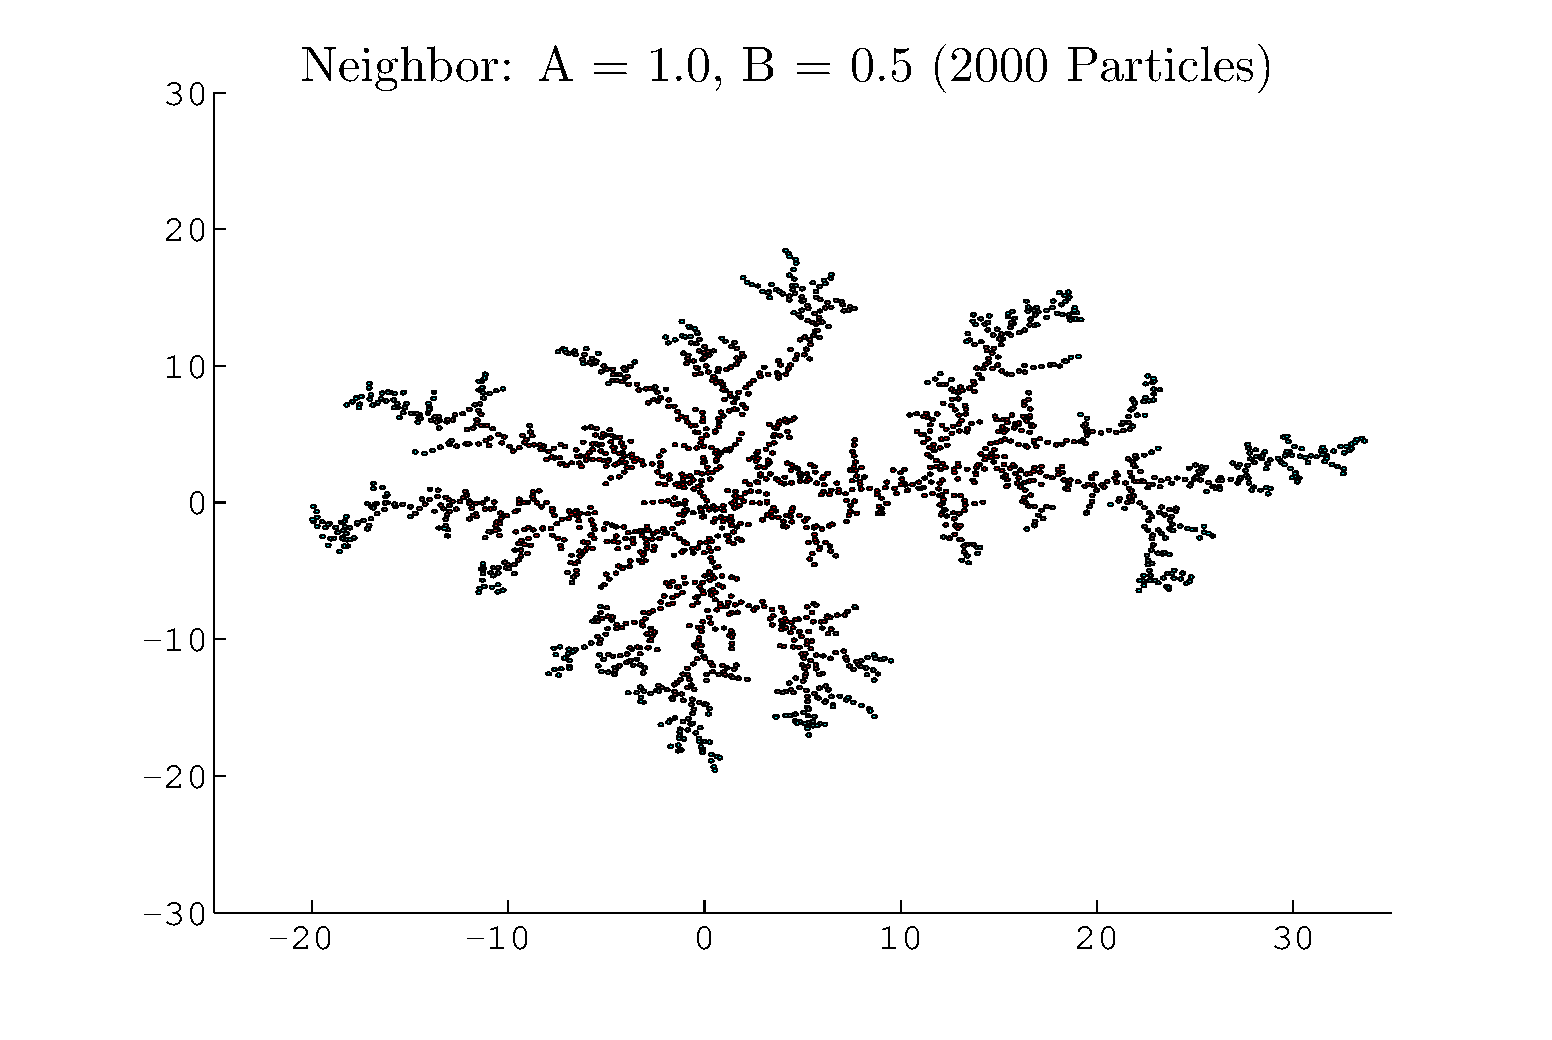
\includegraphics[width=\textwidth]{neigh_1005.eps}
	\caption{DLA simulation for $N=2000$ particles using a neighbor dependent sticking probability (Eq. \ref{p:neighbor}) with A = 1.0 and B = 0.5. }
	\label{fig:neigh}
\end{center}
\end{figure}

\begin{figure}
\begin{center}
	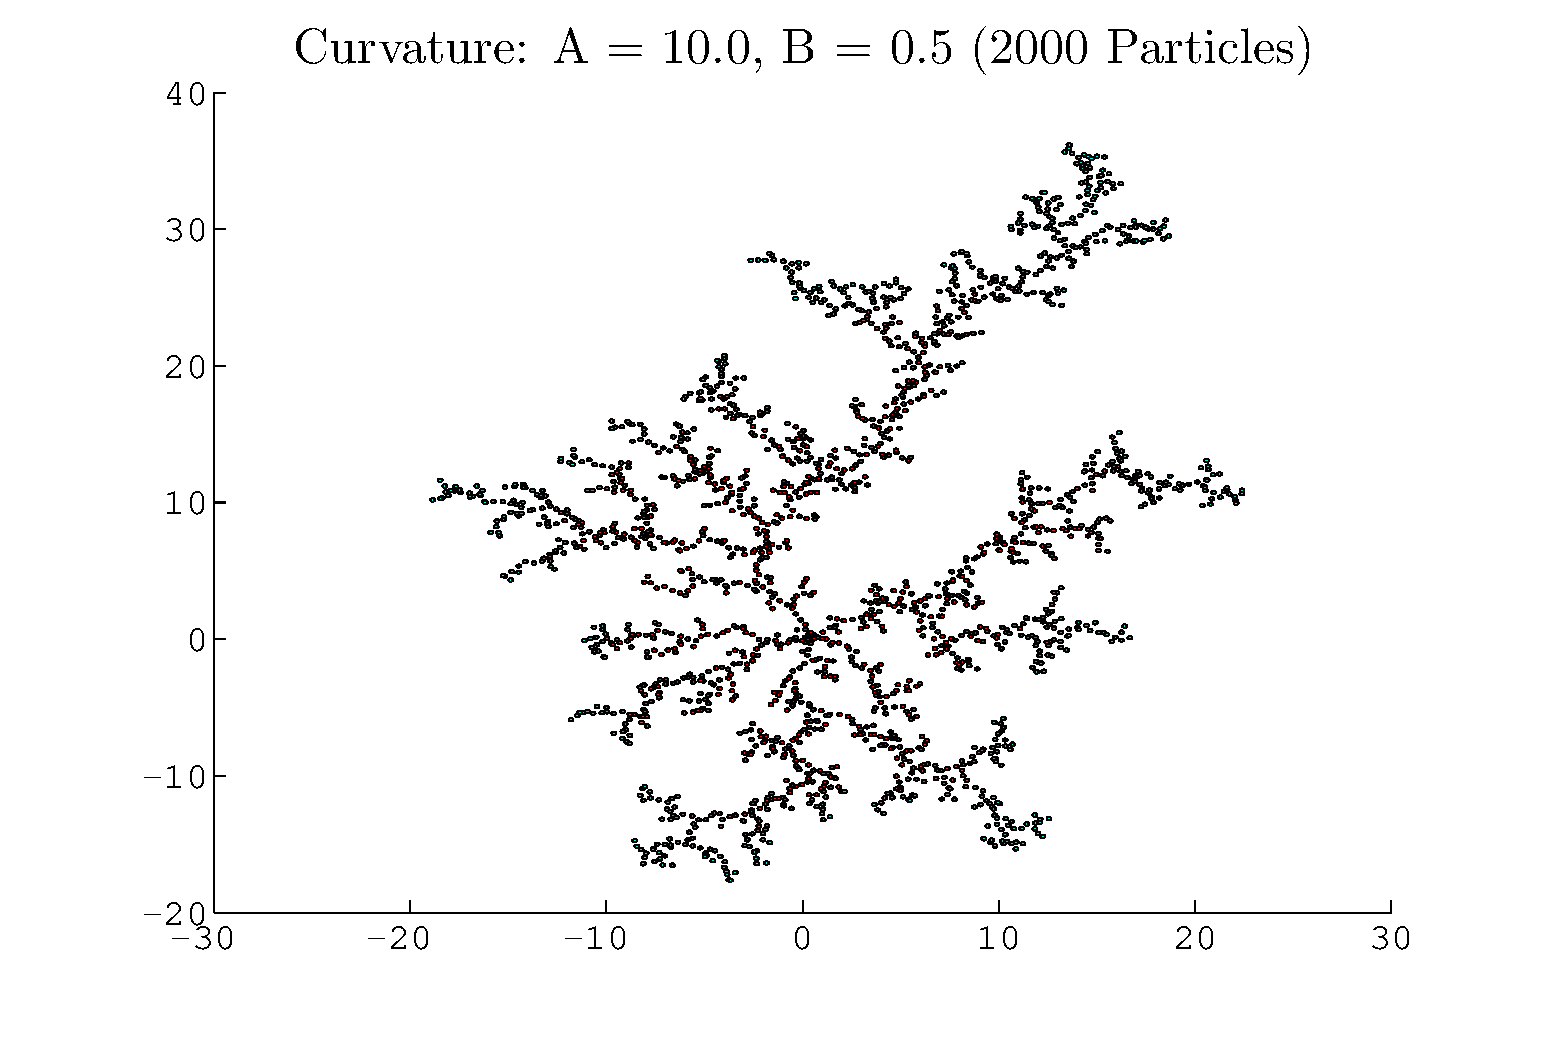
\includegraphics[width=\textwidth]{curve_10005.eps}
	\caption{DLA simulation for $N=2000$ particles using a sticking probability dependent on the local curvature at the point of contact (Eq. \ref{p:curvature}) with A = 10.0 and B = 0.5. }
	\label{fig:curve}
\end{center}
\end{figure}

The sample of aggregates studied were simulations of 1000 particles with constant sticking probabilities given by p = {0.01, 0.1, 0.25, 0.5. 0.75, 1.0}(see Table \ref{tab:dat}). The aggregates were sampled with a constant sticking probability in order to serve a foundation and provide insight into aggregates formed with more complicated sticking probability distributions. The values obtained from these simulation measurements revealed patterns reflecting general attributes of the aggregates. For example, the average distance from the seed particle and the approximate number density  ($\bar{r}$ and $\rho$) are both measures of compactness, and this was generally observed in aggregates with  low $\bar{r}$ and high $\rho$. Additionally, the measure of circularity, which was found by approximating the aggregate as a 12-sided polygon and comparing its perimeter to its area, showed the relative circular symmetry of the aggregate, and aggregates with circularities under 0.5 tended to have significant branching in one or two particular directions (comparing the relative percentage of the maximum distance to the average distance $\frac{r_{max}}{\bar{r}}$ was also indicative of the magnitude of the largest branch). Lastly the measure of characteristic length, which was the average displacement due to diffusion for some given time interval was used to calculate the fractal dimension according to the formula:

\begin{equation}
	D = \frac{\log{N}}{\log{L_{char}}}
\label{eq:fd}
\end{equation}

Fractal dimension is a measure of how ``filled in'' an object is and because these aggregates lie in only 2 dimensions their fractal dimension is somewhere between 1 and 2. Figure \ref{fd_P} plots the fractal dimension as a function of various sticking probabilities. Interestingly, however, the results across all probability functions (greater than about .2) show that the fractal dimension is approximately constant with a value generally around 1.38\footnote{ Note that in Figure \ref{fd_P}, the first two points are marked as outliers. This is due to the earlier oversight of allowing particles to overlap, thus making these points unrepresentative of the true relationship between fractal dimension and sticking probability. Note as well, though, that even despite this source of error, the approximate fractal dimension is still relatively constant.}.

\begin{figure}[ht!]
\begin{center}
	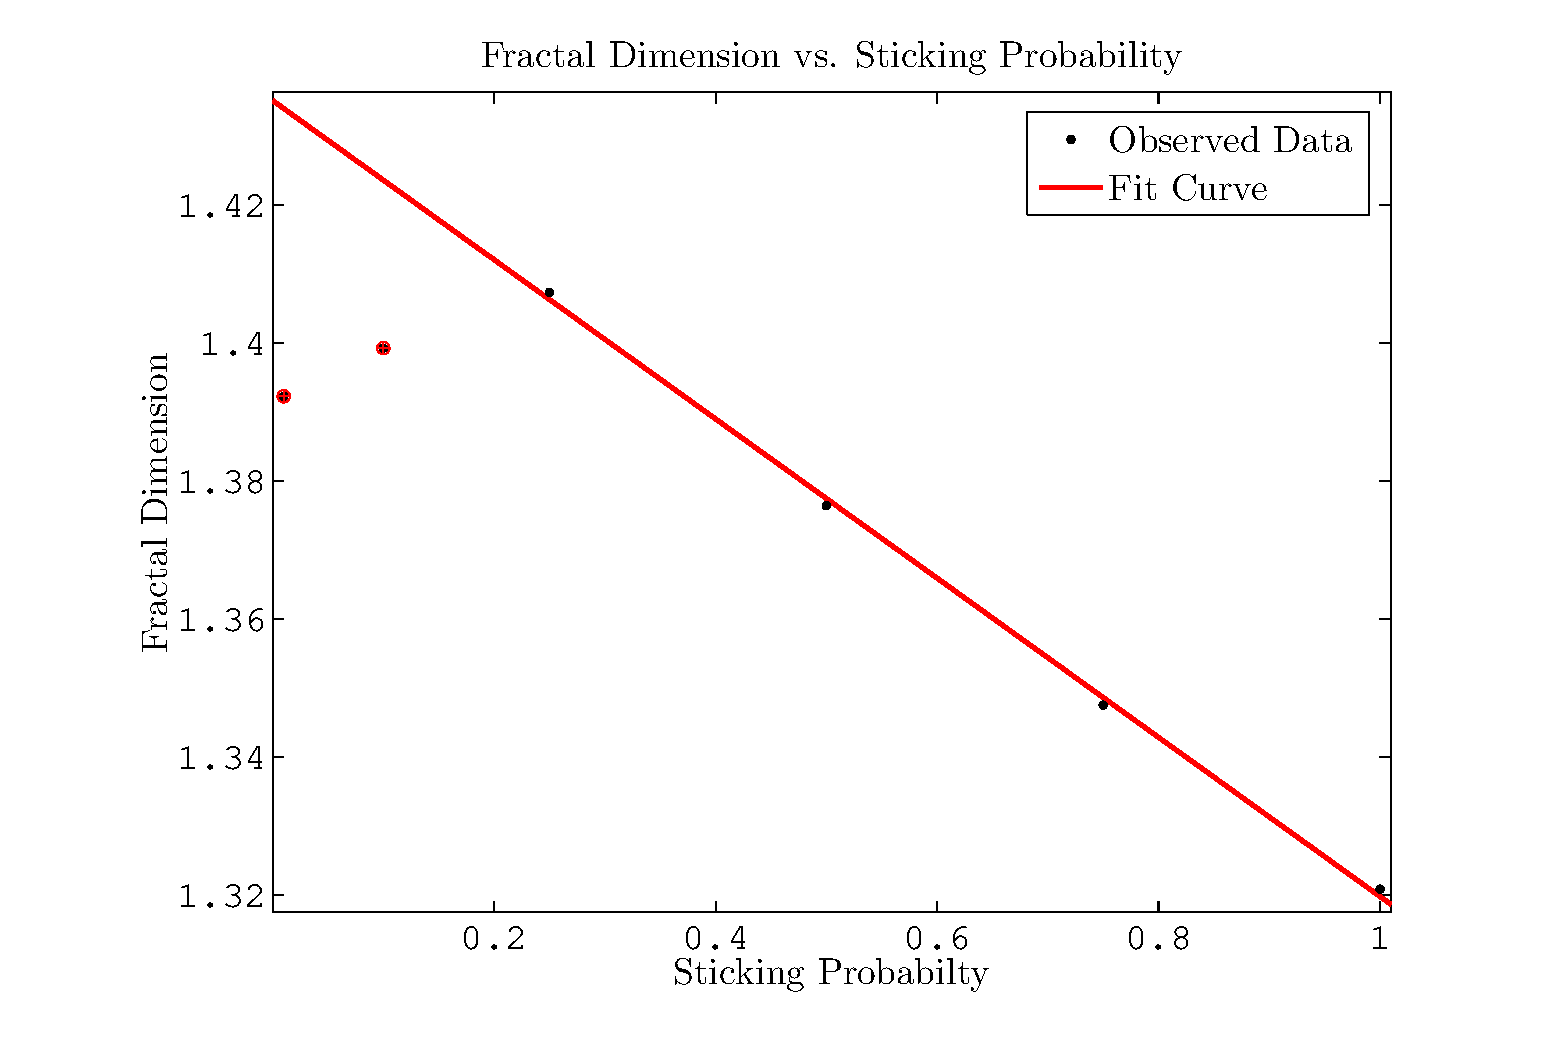
\includegraphics[width=\textwidth]{fd_p.eps}
	\caption{A plot of fractal dimension as a function of sticking probability. Data was gathered from Table \ref{tab:dat}.}
	\label{fd_P}
\end{center}
\end{figure}


This brings up an important finding about the nature of these measurements: due to the high degree of statistical uncertainty that these aggregates are subject to, these measurements of average distance, density, fractal dimension and circularity are not conclusive on their own. While they serve as a quantitative and useful means of comparing various characteristics of these aggregates, the information they convey is insufficient to try and define classes of aggregates or to even develop any significant form of categorization. This issue manifests itself in all the measurements presently recorded. For example, while it may be possible to say that the observed aggregates formed with a sticking probability of $p = 0.25$ had an average density of $26.04 \pm 1.9$, circularity of $0.76 \pm .07$, average distance of $6.21 \pm 0.21$ and fractal dimension of about 1.41 it is impossible to say that any aggregate (or even most of the aggregates) I observe with similar parameters were formed with a sticking probability of 0.25 (or something close), and this is simply because there is too much uncertainty and overlap with other probabilities (due to the random nature of DLA). Thus in order to create any meaningful categorization of these aggregates, other parameters must be sought out as well. Since the ones used in this study were the simplest to calculate, a fully definitive set of categorization may be a complex system to develop.




%----------------------------------------------------------------------------------------
%	SECTION 5
%----------------------------------------------------------------------------------------

\section{Conclusions: \label{conclusions}}

The results of this DLA simulator are clear, and despite being slightly oversimplified in a few of its assumptions, the aggregates generated are still remarkably similar to the physical aggregates observed in experiments. Additionally, the inclusion of a sticking probability allowed pattern formation in theses aggregates to be studied under various conditions, although it was observed that aggregates formed under higher sticking probabilities were physically more accurate than under low sticking probability conditions.

One of the major secondary objectives of this study was to determine the relevant parameters that characterize an aggregate and furthermore to determine the feasibility of creating classes of aggregate structures. After observing these aggregates being formed under various conditions, only a few relevant parameters were determined, these being fractal dimension, number density, mean radius, and circularity. In conjunction with one another, these values give reasonable insight into the distribution of the aggregate members, and we can begin to see relationships between these values and certain patterns in the aggregate structure. These different parameters create a means of studying and comparing different aggregates. As a method of classifying these aggregates, however, they are insufficient. For example, Figure \ref{fd_P} showed that on average as the sticking probability varied (occasionally resulting in dramatically different aggregate patterns) the fractal dimension remained relatively constant, despite being a relevant characterization parameter. Thus, patterns formed in DLA structures are subject to an overwhelming amount of statistical variation and the aggregates observed in these simulations would blur over any hard definitions formed on these parameters alone. 

One potential source of the statistical homogeneity of these aggregates not accounted for in this simulation was the lack of anisotropy during the binding process. In this simulation, this was a result of the continuous and circular symmetry present in the particle motion and binding process. Simulators built on the geometry of a square or hexagonal lattice, for example, have observed various symmetries, which can be attributed restricted nature of the particle behavior in these simulations \cite{vic} \cite{goodflake}. Therefore the comparison of the resulting symmetries between aggregates formed on various lattice geometries may be an interesting point of further research, and could potentially be an additional relevant parameter in characterizing an aggregate. 



%----------------------------------------------------------------------------------------
%	BIBLIOGRAPHY/REFERENCES
%----------------------------------------------------------------------------------------
\pagebreak

\bibliographystyle{plain}

\nocite{*}

\bibliography{refs}

%----------------------------------------------------------------------------------------
%----------------------------------------------------------------------------------------
%	SECTION 6
%----------------------------------------------------------------------------------------

\begin{appendix}

\appendixpage
%\section{Additional Figures: \label{add_figs}}

\section{Bias: \label{bias}}

	The bias parameter was initially included as a means of speeding up the convergence of walker particles towards the aggregate, however, it is observed to have physical implications as well. The bias parameter is controls the magnitude of a constant displacement towards the origin that is added to the net displacement at each step. Thus, the bias simulates the effect of having a constant radial force which attracts the walkers. 
	
\begin{figure}[ht!]
\centering
\begin{subfigure}{.5\textwidth}
  \centering
  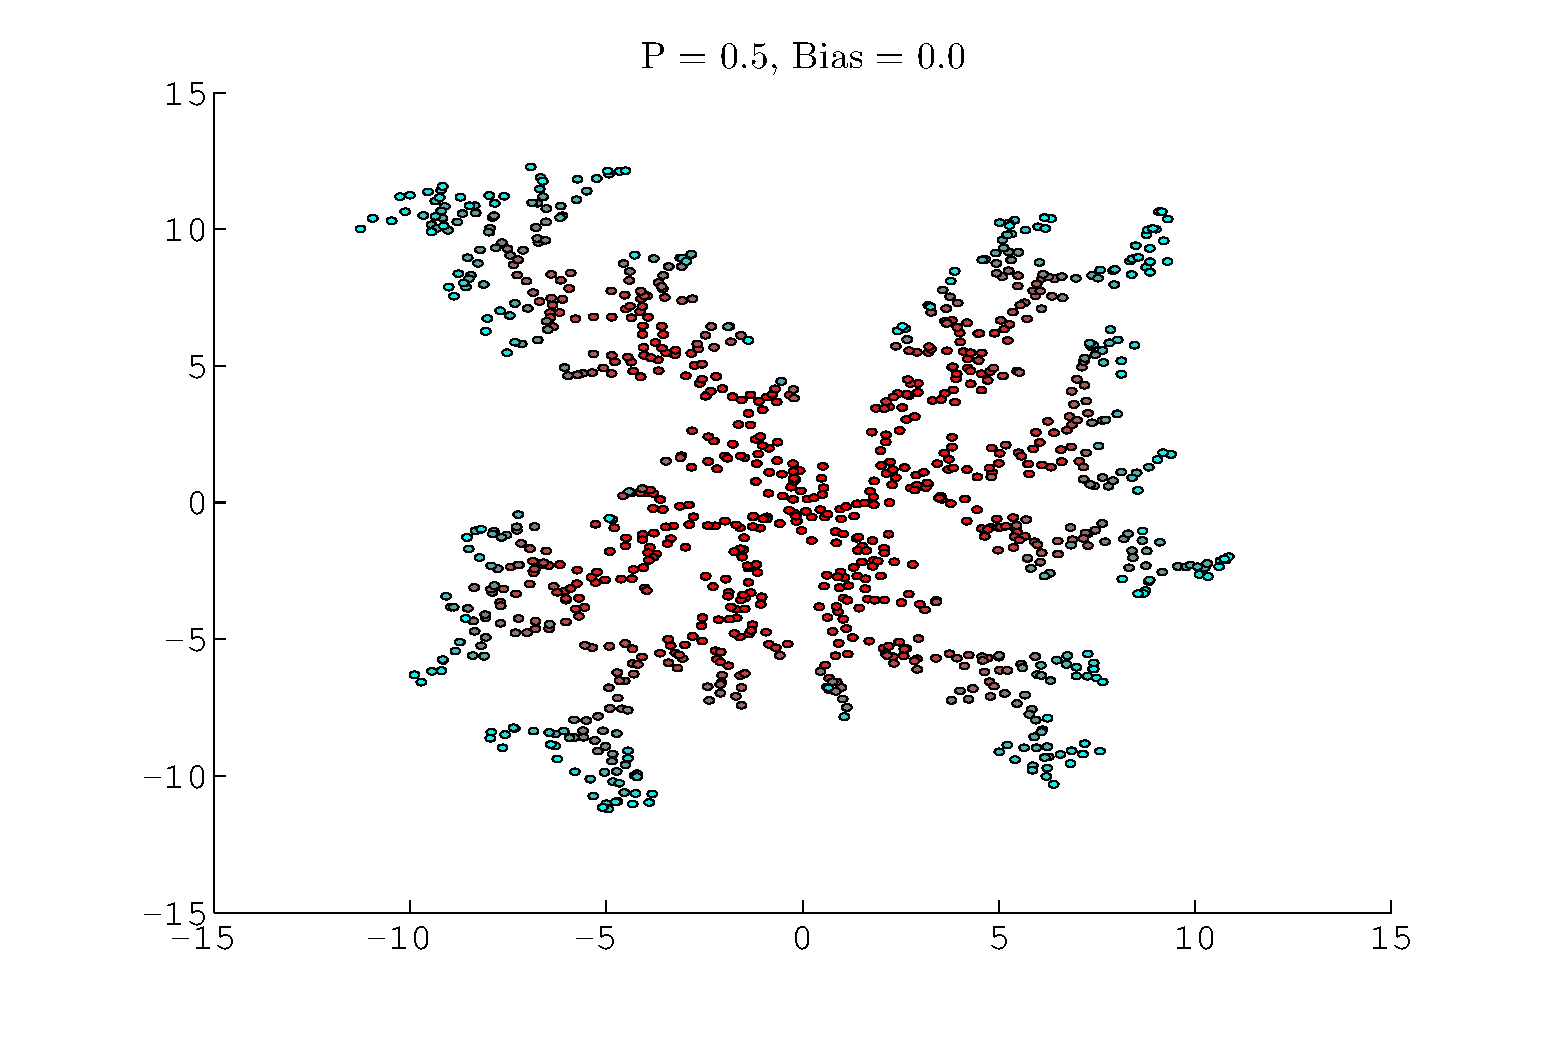
\includegraphics[width=.95\linewidth]{bias_0005.eps}
  \caption[width = .95\linewidth]{Bias = 0.0}
  \label{bias1}
\end{subfigure}%
\begin{subfigure}{.5\textwidth}
  \centering
  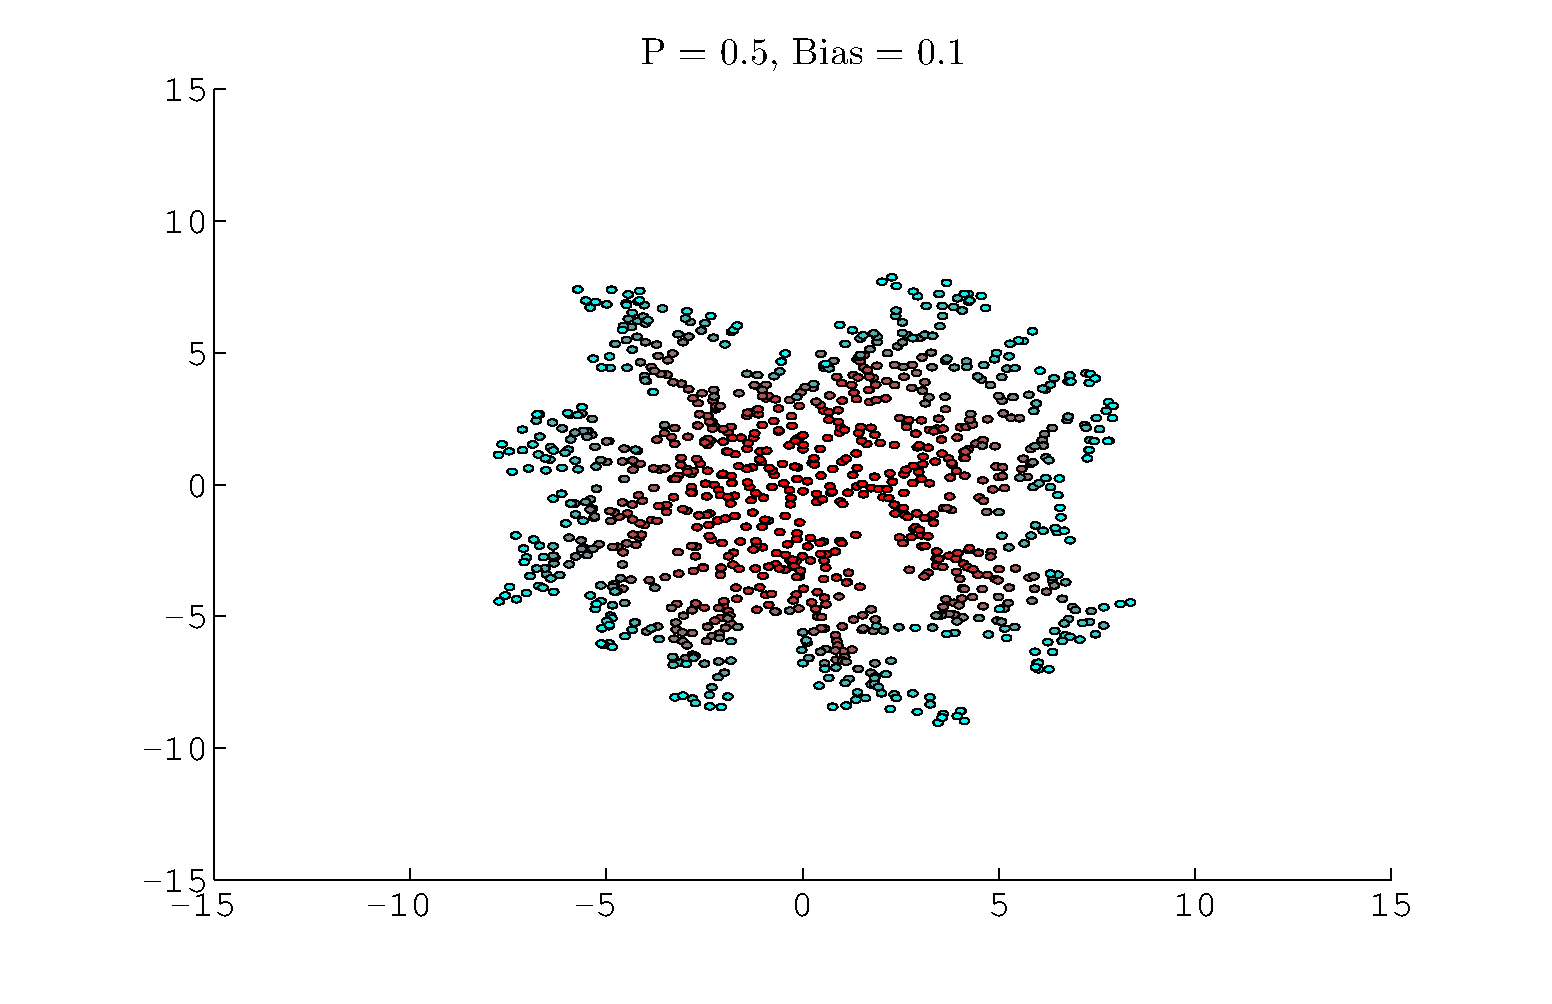
\includegraphics[width=.95\linewidth]{bias_0105.eps}
	\caption[width = .95\linewidth]{Bias = 0.1}
  \label{bias2}
\end{subfigure}
\caption{Comparison of the effects of the bias parameter. In both cases, aggregates were grown with constant sticking probability $p = 0.5$. Notice how, with a bias applied, aggregate members are more evenly distributed throughout the occupied area and the overall distribution is more compact. Simulated for $N = 1000$ particles.}
\label{fig:bias}
\end{figure}

As Figure \ref{fig:bias} shows, the inclusion of even a slight bias has immediately noticeable effects on the particle distribution within the aggregate. The most immediate observation is the lack of branching, a feature that is much more apparent in the Bias = 0 simulation. Further characterizing these two aggregates, other noticeable differences present themselves, such as the the compactness of the aggregate in \ref{bias2} (given by average distance $\bar{r} = 5.1$ and particle density $\rho = 37.1$ compared to $\bar{r} = 7.3$ and $\rho = 18.6$ for \ref{bias1}). Additionally, the circularity of the aggregate in \ref{bias2} is 0.92 whereas the circularity for \ref{bias1} is 0.70. These, stark differences in values for these aggregates show that the effects of even a slight bias are significant.Even in terms of processing time and convergence speed, the bias parameter significantly increased the convergence speed of the algorithm reducing the total number of iterations from 373,976 (with no bias) down to 43,419 (with slight bias).

The effect of this bias parameter opens the door to further topics to explore in future implementations of this simulation. For example, it would be quite interesting to study DLA in the presence of other field geometries, such aggregation in the presence of a tangential force (in the $\hat{\theta}$ direction as opposed to force in the currently implemented $\hat{r}$ direction) which could lead to spiral-like patterns. 

\section{Sample Data and Calculations: \label{data}}

The following data presented in Table \ref{tab:dat} was collected by simulating aggregates constructed using a range of constant sticking probabilities. Each aggregate was simulated for $N = 1000$ particles and only the average values of each measurement are presented in the table. The values measure are:

\begin{description}
	
	\item[Mean Distance ($\bar{r}$):] \hfill \\
	The average distance of each particle from the origin.
	
	\item[Average Collision or Binding Time ($\bar{t_{coll}}$):] \hfill \\
	The average time a particle diffuses until it binds to the aggregate. 
	
	\item[Maximum Distance ($r_{max}$):] \hfill \\
	The farthest distance a particle was from the origin.
	
	\item[Circularity:] \hfill \\
	A measure of the compactness and symmetry of the aggregate.
	
	\item[Characteristic Length:] \hfill \\
	The average displacement of a Brownian particle after an interval $t_{coll}$.
	
\end{description}

\noindent These measurements are relatively straightforward to compute from the aggregate's data, however, characteristic length and circularity will be explained further.

Characteristic length is relatively simple to compute, however, in order to determine the average distance a particle diffuses in $t_{coll}$ a simulation of thousands of Brownian particles was done (see header file r\_walk.h in Appendix \ref{source}).

The calculation of circularity is a bit more involved, requiring one to fit a polygon (arbitrarily chosen to have 12-sides, but accuracy increases with more sides) and to calculate the the perimeter ($L$) and area ($A$) of the fit polygon. Then circularity is: 

\begin{equation}
	4\pi\frac{A}{L^2} \leq 1
\label{eq:circ}
\end{equation}

\noindent A visual representation of this calculation in shown in Figure \ref{circ}. 
\pagebreak


\begin{figure}[ht!]
\begin{center}
	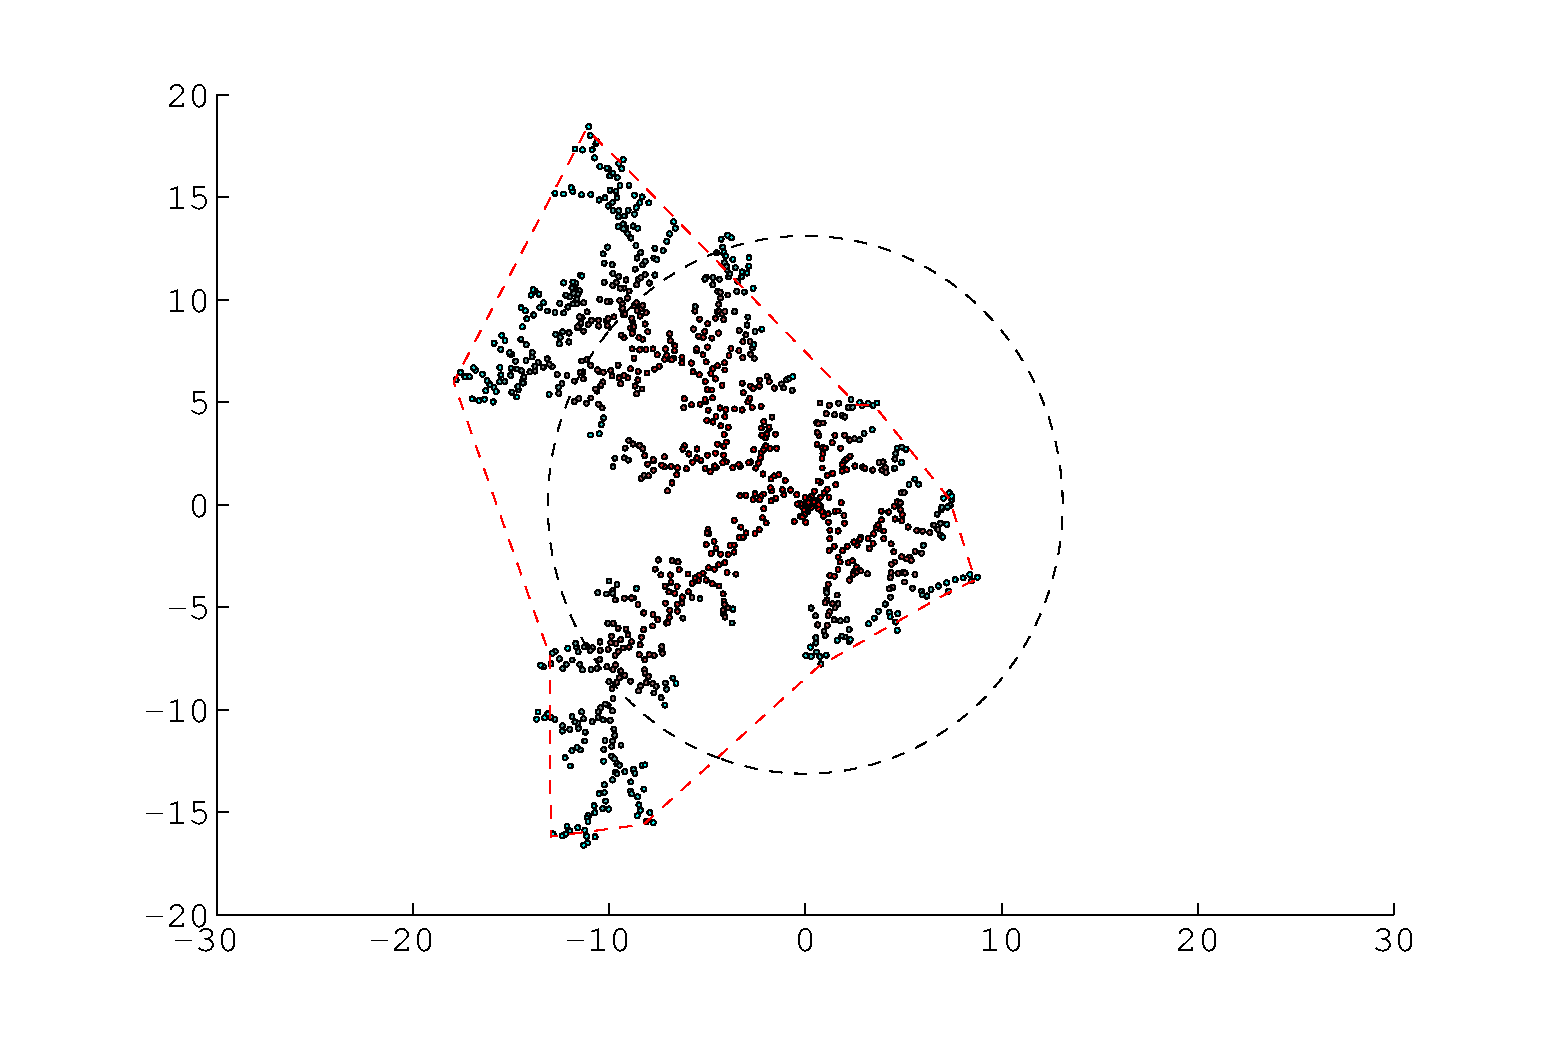
\includegraphics[width=\textwidth]{circ.eps}
	\caption{A visual representation of the calculation of circularity. The perimeter and area of the 12-sided polygon used in Eq. \ref{eq:circ}. This calculation essentially computes the relative similarity between the spanning polygon (red dashed line) and the circle with $r = \bar{r}$ (black dashed line).}
	\label{circ}
\end{center}
\end{figure}

\pagebreak


\begin{sidewaystable}[ht!]
  \centering
  \caption{Sample DLA Data Collected:}
    \begin{tabular}{rrrrrrrrr}
    \toprule
    \multicolumn{4}{c}{p = 0.01}  & \multicolumn{1}{c}{} & \multicolumn{4}{c}{p = 0.5} \\
    \midrule
          &       & Mean  & St. Dev. &       &       &       & Mean  & St. Dev. \\
    $\bar{r}$   &       & 1.878887 & 0.181816 &       & $\bar{r}$   &       & 7.562778 & 0.415017 \\
    $\bar{t_{coll}}$   &       & 82474.82 & 13725.67 &       & $\bar{t_{coll}}$   &       & 93528.33 & 36828.52 \\
    Density &       & 290.26 & 53.83976 &       & Density &       & 17.62005 & 1.865095 \\
    rmax  &       & 4.745631 & 0.52132 &       & rmax  &       & 16.00884 & 1.536601 \\
    Circularity &       & 0.807827 & 0.056796 &       & Circularity &       & 0.691915 & 0.072349 \\
    Characteristic Length & 142.79 &       &       &       & Characteristic Length & 151.19 &       &  \\
          &       &       &       &       &       &       &       &  \\
    \midrule
		\multicolumn{4}{c}{p = 0.1}   & \multicolumn{1}{c}{} & \multicolumn{4}{c}{p = 0.75} \\
    \midrule
					&       & Mean  & St. Dev. &       &       &       & Mean  & St. Dev. \\
    $\bar{r}$   &       & 4.614607 & 0.175134 &       & $\bar{r}$   &       & 8.501541 & 0.403492 \\
    $\bar{t_{coll}}$   &       & 78262 & 18361.7 &       & $\bar{t_{coll}}$   &       & 111973.3 & 28866.56 \\
    Density &       & 47.1379 & 3.491457 &       & Density &       & 13.88823 & 1.234468 \\
    rmax  &       & 10.62307 & 0.968741 &       & rmax  &       & 17.88367 & 1.007205 \\
    Circularity &       & 0.720795 & 0.118113 &       & Circularity &       & 0.684356 & 0.136055 \\
    Characteristic Length & 139.3 &       &       &       & Characteristic Length & 168.37 &       &  \\
          &       &       &       &       &       &       &       &  \\
    \midrule
		\multicolumn{4}{c}{p = 0.25}  & \multicolumn{1}{c}{} & \multicolumn{4}{c}{p = 1.0} \\
    \midrule
					&       & Mean  & St. Dev. &       &       &       & Mean  & St. Dev. \\
    $\bar{r}$   &       & 6.206999 & 0.211136 &       & $\bar{r}$   &       & 9.394982 & 0.833224 \\
    $\bar{t_{coll}}$   &       & 74976.1 & 23724.19 &       & $\bar{t_{coll}}$   &       & 138017.6 & 68030.42 \\
    Density &       & 26.04078 & 1.863252 &       & Density &       & 11.54414 & 1.765577 \\
    rmax  &       & 13.42167 & 0.852675 &       & rmax  &       & 20.31463 & 3.087495 \\
    Circularity &       & 0.763463 & 0.068235 &       & Circularity &       & 0.750503 & 0.083498 \\
    Characteristic Length & 135.39 &       &       &       & Characteristic Length & 186.74 &       &  \\
    \bottomrule
    \end{tabular}%
  \label{tab:dat}%
\end{sidewaystable}%



\section{Source Code Listings: \label{source}}
	
	\lstinputlisting[language=C++]{Final.cpp}

	\lstinputlisting[language=C++]{p_coeff.h}

	\lstinputlisting[language=C++]{p_neighbors.h}

	\lstinputlisting[language=C++]{p_curvature.h}

	\lstinputlisting[language=C++]{r_walk.h}
\end{appendix} 


%----------------------------------------------------------------------------------------

\end{document}